\documentclass[aspectratio=169]{beamer}
\usepackage[utf8]{inputenc} % codificacao de caracteres
\usepackage[T1]{fontenc}    % codificacao de fontes
\usepackage[english]{babel}  % idioma
\usepackage{graphics,amssymb,amsfonts,amsmath,xfrac}
\usepackage{tikz}
\usepackage{enumerate,hyperref}
\usepackage{palatino}	% Fonte sem serifa
\usepackage{ragged2e}	% Paragrafo justificado
%\usepackage{minted}	% Highlight para codigos de programacao
\usepackage{booktabs} % tabelas
\usepackage{multicol}
\usepackage{multirow}
\usepackage{mathrsfs}
\usepackage{relsize}


%\usepackage[table]{xcolor}
\newcommand{\Laplace}[1]{\ensuremath{\mathcal{L}{\left[#1\right]}}}
\newcommand{\InvLap}[1]{\ensuremath{\mathcal{L}^{-1}{\left[#1\right]}}}

% Veja mais temas e cores em http://www.hartwork.org/beamer-theme-matrix/
\usetheme{Montpellier}         % tema
\usecolortheme{orchid}      % cores
\usefonttheme[onlymath]{serif} % fonte modo matematico
% Colocando numero de paginas no slide
\setbeamertemplate{footline}[frame number]



\DeclareGraphicsExtensions{.pdf,.JPG,.png} % compilamos apenas com pdflatex
%\graphicspath{{./figuras/}} % caminho onde as figuras estarao disponiveis


\graphicspath{{figuras/}}

% ---------------------------------------------------------------------------- %
% T�tulo                                                                       %
% ---------------------------------------------------------------------------- %

\title[\sc{Teoria de Circuitos Eletrônicos 1}]{\LARGE Aula 13 - Sinusoidal Steady - State Analysis}
\author[Prof. Marcelino Andrade]{Prof. Marcelino Andrade}
\institute{Faculdade UnB Gama} % opcional
\date{\today}

\begin{document}
\justifying % Paragrafo justificado
\pagebreak

\begin{frame}
  \titlepage
\end{frame}


% ----------------- NOVO SLIDE --------------------------------
\begin{frame}{Contents}

\tableofcontents
%\begin{center}	
     		Introduction to Electric Circuits by James A. Svoboda, Richard C. Dorf, 9th Edition 
  %   		Fundamentals of Electric Circuits by Alexander and Sadiku, 4th Edition	
%\end{center}	
\end{frame}

% ----------------- NOVA SECÇÂO -----------------------------
\section{Introduction (10.1)}
% ----------------- NOVO SLIDE --------------------------------
\begin{frame}[fragile]
	\frametitle{Introduction}
		\begin{tabular}{cc}
		
		
			\begin{columns}
	\small			\begin{column}{1\textwidth}  %%<--- here
Linear circuits with sinusoidal inputs that are at steady state are called ac circuits. The electric
power system that provides us with convenient electricity is a very large ac circuit. AC circuits are the
subject of this chapter. In particular, we will see that: 	
						
				\end{column}
			\end{columns}\\
		
		
		
			\begin{columns}
\small				\begin{column}{.5\textwidth}  %%<--- here
	
		
		\begin{itemize}
						\item[$\clubsuit$]{It’s useful to associate a complex number with a sinusoid. Doing so allows us to define phasors
and impedances.}
						\item[$\clubsuit$]{Using phasors and impedances, we obtain a new representation of the linear circuit, called the
“frequency-domain representation.”}
						\item[$\clubsuit$]{We can analyze ac circuits in the frequency 
						domain to determine their steady-state response.}		
	
					\end{itemize}
					
				\end{column}
				\begin{column}{.5\textwidth}  %%<--- here
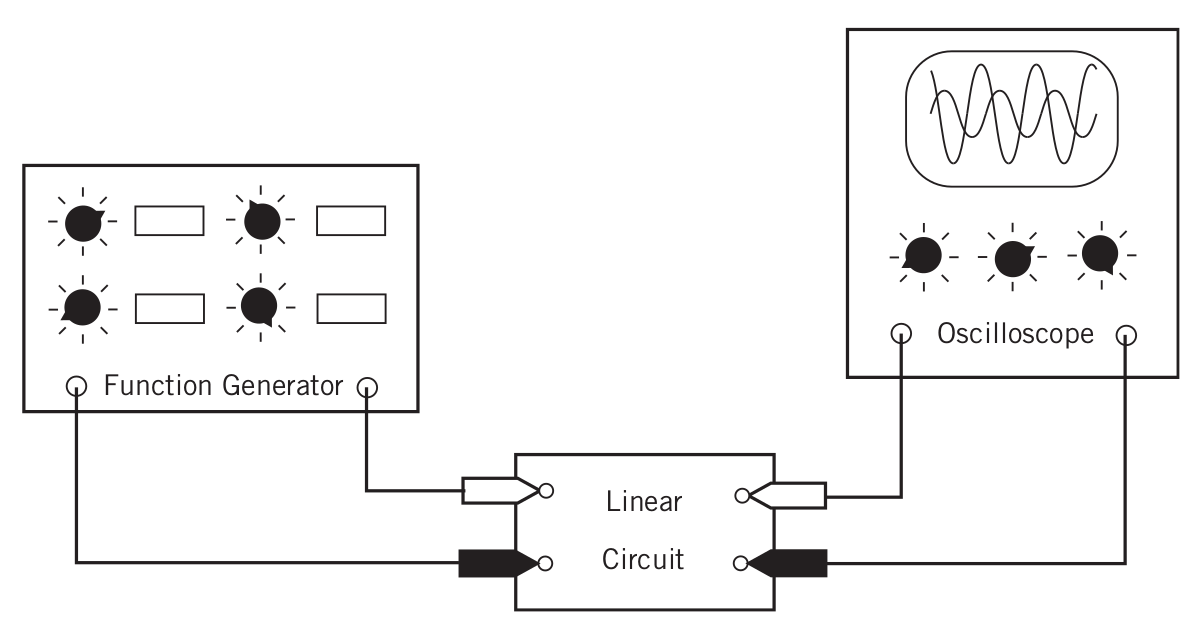
\includegraphics[height=3.5cm]{figure1.png}	
					
				\end{column}
			\end{columns}
		
	\end{tabular}
\end{frame}

% ----------------- NOVA SECÇÂO -----------------------------
\section{Sinusoidal Sources (10.2)}
% ----------------- NOVO SLIDE --------------------------------
\begin{frame}[fragile]
	\frametitle{Phase Advance and Delay}
		\begin{tabular}{cc}

	\begin{columns}
	\begin{column}{.5\textwidth}  %%<--- here
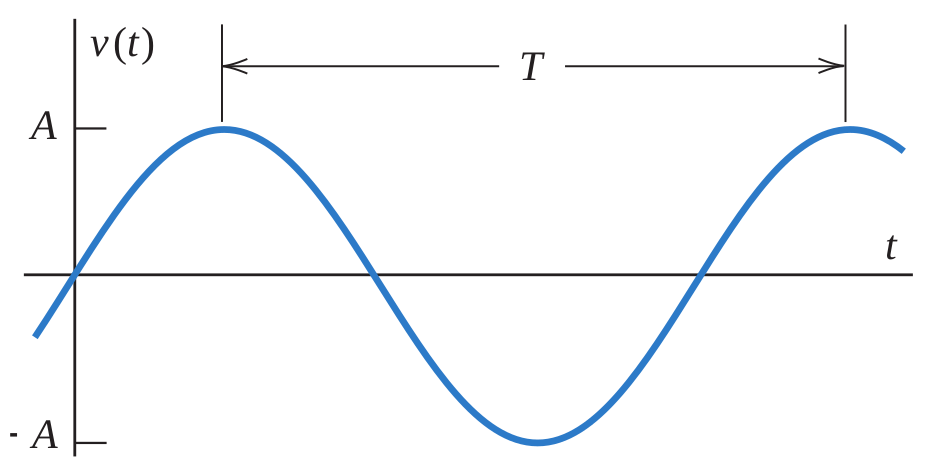
\includegraphics[width=6cm,height=2.85cm]{figure2.png}\\
		$v(t)= \sin (\omega t)$\\
		$v(t)=v(t+T)$\\
		$f=\dfrac{1}{T}$\\
		$\omega = 2 \pi f = \dfrac{2 \pi}{T}$\\

 
				\end{column}
\begin{column}{.5\textwidth}  %%<--- here\
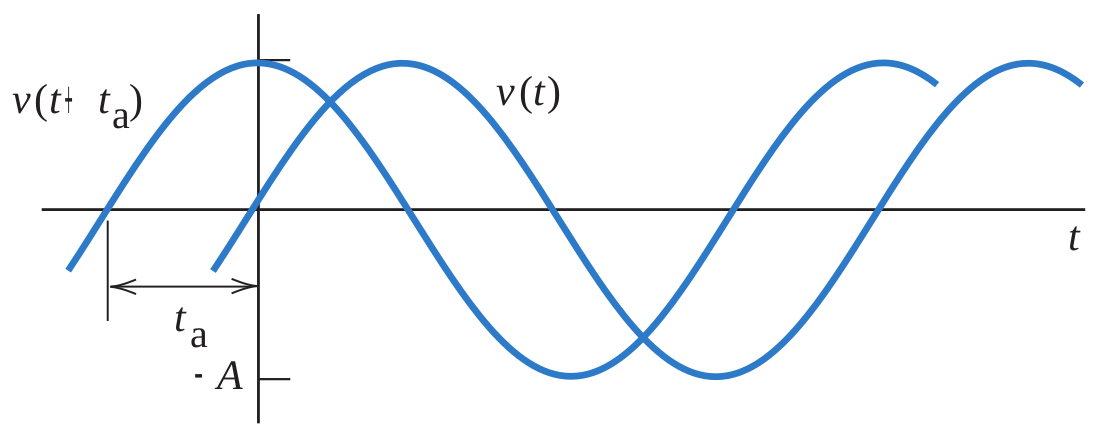
\includegraphics[width=6cm,height=2.5cm]{figure3.png}\\
		$v(t+t_a)= \sin (\omega (t+t_a))=\sin (\omega t+ \omega t_a)$\\
		$v(t+t_a)=\sin (\omega t+ \theta )$ \\
\scriptsize		The phase angle in radians is related to
the time $t_a$ by \\
\normalsize		$\theta= \omega t_a = \dfrac{2 \pi}{T} t_a$\\
\scriptsize	An advance by time $t_a$ is equivalent $T+t_a$. Similarly, a delay by time $t_d$
is equivalent  $T-t_d$.
				\end{column}				
	\end{columns}\\	
			
			
				
				
				
	\end{tabular}		
\end{frame}



% ----------------- NOVA SECÇÂO -----------------------------

\section{Phasors and Sinusoids (10.3)}
% ----------------- NOVO SLIDE --------------------------------
\begin{frame}[fragile]
	\frametitle{Phasors and Sinusoids}
\begin{tabular}{ll}

	\begin{columns}
\scriptsize		\begin{column}{0.5\textwidth}  %%<--- here
A phasor is a complex number that is used to represent the amplitude and phase angle of a
sinusoid. The relationship between the sinusoid and the phasor is described by

$$A \cos(\omega t + \theta) \leftrightarrow A \angle{\theta}$$ 
There are a couple of things that we should notice.
\begin{itemize}
						\item[$\clubsuit$]{The sinusoid is represented using the cosine
rather than the sine function.}
						\item[$\clubsuit$]{the phasor is a complex number represented in polar form.}
						\item[$\clubsuit$]{The
magnitude of the phasor is equal to the amplitude of the sinusoid, and the angle of the phasor is equal to
the phase angle of the sinusoid.}		
	
					\end{itemize}
		\end{column}
		\begin{column}{0.5\textwidth}  %%<--- here
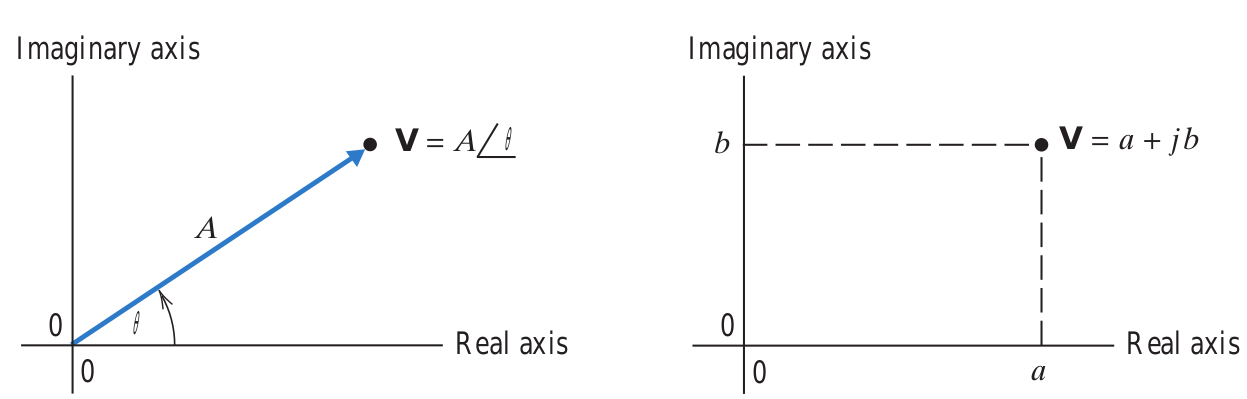
\includegraphics[width=7cm,height=2.5cm]{figure4.png}\\
To indicate that A is the
magnitude of the phasor V and that y is the angle of V, we write \\
	$A=|\textbf{V}| \ and \ \theta=\angle{\textbf{V}}$\\
	$a= Re(\textbf{V}) \ and \ b=Im(\textbf{V})$\\
		$\textbf{V}=a+jb$\\
		Since a phasor can be expressed in both rectangular and polar forms, we write\\
		$\textbf{V} = a+jb = |\textbf{V}|\angle{\textbf{V}}= A\angle{\theta}$\\
		$\omega = 2 \pi f = \dfrac{2 \pi}{T}$\\
		\end{column}
	\end{columns}\\	
\end{tabular}
\end{frame}
% ----------------- NOVO SLIDE --------------------------------
\begin{frame}[fragile]
	\frametitle{Phasors and Sinusoids}
\begin{tabular}{ll}

	\begin{columns}
\scriptsize		\begin{column}{0.5\textwidth}  %%<--- here
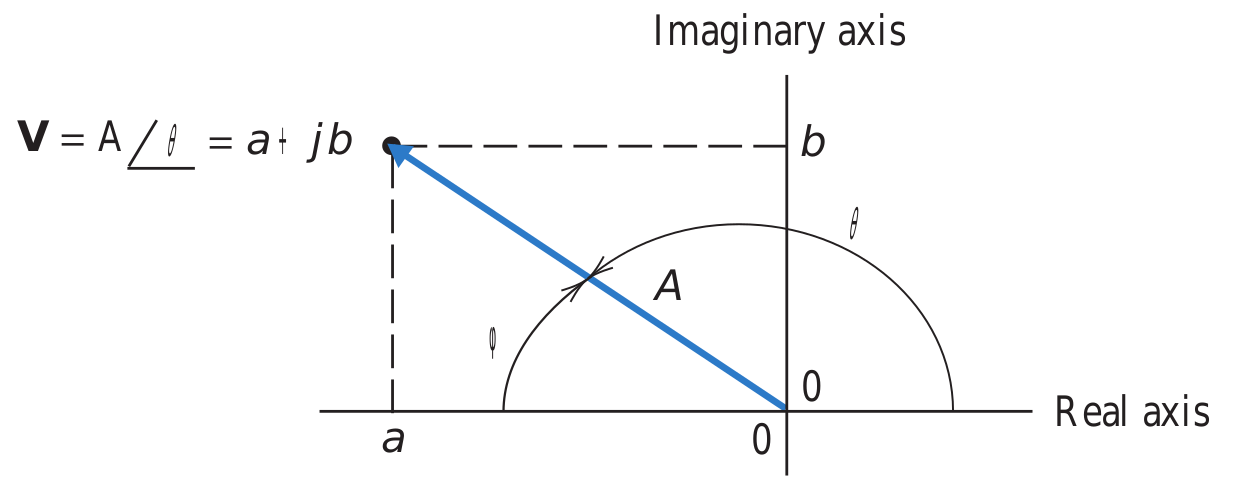
\includegraphics[width=7cm,height=2.5cm]{figure5.png}\\
The trigonometry provides the following equations for converting
between the rectangular and polar forms of phasors.\\
	$a= \cos(\theta), \ b= A \sin(\theta), \ A=\sqrt{a^2+b^2}$ \newline \\ and \ 
$
	    \theta=
	    \begin{cases}
	    \tan^{-1}(\dfrac{b}{a}), \ when \ a > 0 \\
	%    \newline \\
	    180^o-\tan^{-1}(\dfrac{b}{-a}), \ when \ a < 0 \\
	    
	    \end{cases}
	    $
		\end{column}
		\begin{column}{0.5\textwidth}  %%<--- here
The use of phasors to represent sinusoids is based on Euler’s formula. Euler’s formula is \newline \\
 $e^{j \phi}= \cos(\phi)+j \sin(\phi)$ \newline \\
 Consequently,\newline \\
  $Ae^{j \phi}= A\cos(\phi)+j A\sin(\phi)=A \angle{\phi}$ \newline \\
    $Ae^{j \phi}=A \angle{\phi}$ \newline \\
 $Ae^{j \phi}$ is called the exponential form of a phasor. \newline \\
 
 The conversion between the polar and exponential
forms is immediate. In both, A is the amplitude of the sinusoid and $\phi$ is the phase angle of the sinusoid.
		\end{column}
	\end{columns}\\	
\end{tabular}
\end{frame}
% ----------------- NOVO SLIDE --------------------------------
\begin{frame}[fragile]
	\frametitle{Phasors and Sinusoids}
\begin{tabular}{ll}

	\begin{columns}
\scriptsize		\begin{column}{1\textwidth}  %%<--- here
 \begin{tabular}{ll}
	\begin{columns}
	\begin{column}{1\textwidth}  %%<--- here
 	$\Rightarrow$ \textbf{EXAMPLE 10.2-1} - Consider the sinusoids $v_1(t)=10 \cos(200t+45^o) V$ and 
$v_2(t)=8 \sin(200t+15^o) V$. Determine the time by which $v_ 2(t)$ is advanced or delayed with respect to $v_1(t)$. \\

\scalebox{0.8}{Answer: $t_d=-10.47ms$}\\
		
		\end{column}
	\end{columns}\\
	\begin{columns}
	\begin{column}{1\textwidth}  %%<--- here
\newline \newline	$\Rightarrow$	\textbf{EXAMPLE 10.3-1} - Determine the phasors corresponding to the sinusoids
$i_1(t)=120 \cos(400t+60^o)mA$ and $i_2(t)=100 \sin(400t-75^o)mA$  \\  \scalebox{0.8}{Answer: $I_1=120 \angle{60^o}$ and $I_2=100 \angle{-165^o}$ }\\
		\end{column}
	\end{columns}\\
	\begin{columns}
		\begin{column}{1\textwidth}  %%<--- here
\newline \newline	$\Rightarrow$		\textbf{EXAMPLE 10.3-2} - Consider the phasors
$\textbf{V}_1=4.25 \angle{115^o}$ and $\textbf{V}_2=-4+j3$. Convert $\textbf{V}_1$ to rectangular form and $\textbf{V}_2$ to polar form. \\
\scalebox{0.8}{Answer:  $\textbf{V}_1 = -1.796+j3.852$ and $\textbf{V}_2=5 \angle{143^o}$ }\\
		
		\end{column}
	\end{columns}\\
	\begin{columns}
		\begin{column}{1\textwidth}  %%<--- here
\newline \newline	$\Rightarrow$		\textbf{EXERCISE 10.3-3} - Consider the phasors $\textbf{V}_1 = -1.796+j3.852=4.25 \angle{115^o}$
	
	and $\textbf{V}_2 = -4+j3=5 \angle{143^o}$. Determine $\textbf{V}_1+\textbf{V}_2$, $\textbf{V}_1.\textbf{V}_2$ and 
	$\frac{\textbf{V}_1}{\textbf{V}_2}$  \\
	\scalebox{0.8}{Answer: $\textbf{V}_1+\textbf{V}_2=-5.796+j6.852$, $\textbf{V}_1.\textbf{V}_2=21.25 \angle{-102^o}$ and 
	$\frac{\textbf{V}_1}{\textbf{V}_2}=0.85 \angle{-28^o}$}\\
		
		\end{column}
	\end{columns}\\
\end{tabular}


\end{column}

	\end{columns}\\	

	
	
\end{tabular}
\end{frame}
% ----------------- NOVO SLIDE --------------------------------
\begin{frame}[fragile]
	\frametitle{KVL or KCL equation from an ac circuit}
\begin{tabular}{ll}

	\begin{columns}
\scriptsize		\begin{column}{0.5\textwidth}  %%<--- here
Consider \newline \\
$e^{\omega t + \theta}= \cos(\omega t + \theta)+j \sin(\omega t + \theta)$ \newline \\ 
Taking the real part of both sides gives \newline \\
$A \cos(\omega t + \theta)=Re \{e^{\omega t + \theta}\}=Re \{e^{\omega t} e^{ \theta}\}$ \newline \\
Consider a sinusoid and corresponding phasor \newline \\
$v(t) = A \cos(\omega t + \theta) V$ and $\textbf{V}(\omega)=A \angle{\theta} = A e^{j \theta}$ \newline \\
$v(t) = Re \{\textbf{V}(\omega) e^{j \omega t}   \}$ \newline \\
		Next, consider a KVL or KCL equation from an ac circuit, for example, \newline \\
$0=\sum_{i} v_i(t) = \sum_{i} Re \{\textbf{V}_i(\omega) e^{j \omega t}   \}= \sum_{i}  Re \{ e^{j \omega t} \textbf{V}_i(\omega)    \}$ \newline \\



		\end{column}
		\begin{column}{0.5\textwidth}  %%<--- here

Eq. before is required to be true for all values of time t. Let t = 0. \newline \\
$0= \sum_{i}  Re \{ \textbf{V}_i(\omega)    \}$ \newline \\
Next, \newline \\
$0= \sum_{i}  Re \{ j \textbf{V}_i(\omega)    \}= \sum_{i}  Im \{  \textbf{V}_i(\omega)    \}$ \newline \\
Together, \newline \\
$0= \sum_{i}  \{ \textbf{V}_i(\omega)    \}$ \newline \\ 
In summary, if a set of sinusoidal voltages $v_i (t)$ satisfy KVL for an ac circuit, the
corresponding phasor voltages $\textbf{V}_i(\omega)$ satisfy the same KVL equation. Similarly, if a set of
sinusoidal currents $i_i(t)$ satisfy KCL for an ac circuit, the corresponding phasor currents $\textbf{I}_i(\omega)$
satisfy the same KCL equation.
\end{column}
	\end{columns}\\	
\end{tabular}
\end{frame}


% ----------------- NOVO SLIDE --------------------------------
\begin{frame}[fragile]
	\frametitle{KVL or KCL equation from an ac circuit}
\begin{tabular}{ll}
\begin{columns}
 \begin{column}{1\textwidth} 
		\textbf{EXAMPLE 10.3-4 Kirchhoff’s Laws for AC Circuits} - The input to the circuit shown in Figure  
is the voltage source voltage,
  
 \end{column}

 
\end{columns}\\



	\begin{columns}
		\begin{column}{.5\textwidth}  %%<--- here


$$v_s(t)=25 \cos(100t+15^o)$$

The output is the voltage across the capacitor,

$$v_C(t)=20 \cos(100t-22^o)$$

Determine the resistor voltage $v_R (t)$. \newline \\
\scalebox{0.8}{Answer: $V_R(t)=15 \cos(100t+68.1^o)$}\\
		\end{column}
		\begin{column}{.5\textwidth}  %%<--- here


\begin{center}
    			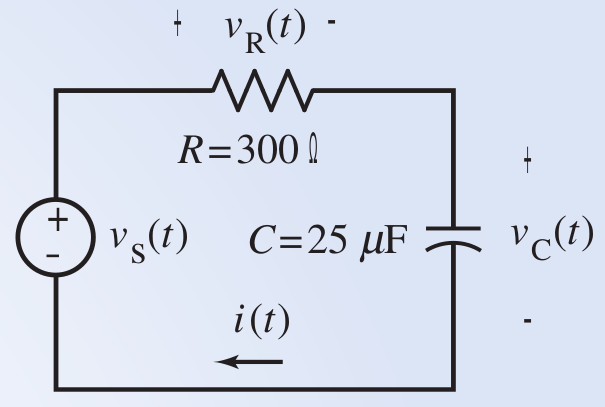
\includegraphics[width=5.5cm,height=4.cm]{figure6.png}	
		\end{center}
		\end{column}
		
	\end{columns}\\
	
	

	
	
\end{tabular}
\end{frame}
% ----------------- NOVA SECÇÂO -----------------------------
\section{Impedances (10.4)}
% ----------------- NOVO SLIDE --------------------------------
\begin{frame}[fragile]
	\frametitle{Impedances}
\begin{tabular}{ll}

	\begin{columns}
\scriptsize		\begin{column}{0.5\textwidth}  %%<--- here
The element voltage and element current are labeled
as v(t) and i(t). We can write \newline \\
$v(t)= V_m \cos(\omega t + \theta) \ V$ and $i(t)= I_m \cos(\omega t + \phi) \ A$ \newline \\ 
The corresponding phasors are \newline \\
$\textbf{V}(\omega)=V_m \angle{\theta} \ V$ and $\textbf{I}(\omega)=I_m \angle{\phi} \ A$\newline \\
The impedance is denoted as $\textbf{Z}(\omega)$ so \newline \\
$\textbf{Z}(\omega)=\dfrac{\textbf{V}(\omega)}{\textbf{I}(\omega)}=\dfrac{V_m \angle{\theta}}{I_m \angle{\phi}}=\dfrac{V_m}{I_m}\angle{(\theta-\phi)}$ \newline \\
The admittance is denoted as $\textbf{Y}(\omega)$ so \newline \\
$\textbf{Y}(\omega)=\dfrac{\textbf{I}(\omega)}{\textbf{V}(\omega)}$ \newline \\


		\end{column}
		\begin{column}{0.5\textwidth}  %%<--- here

Consequently, \newline \\
$\textbf{V}(\omega)={\textbf{Z}(\omega)}{\textbf{I}(\omega)}$ \newline \\
which is \textbf{Ohm’s law for ac circuits}. \newline \\
\center 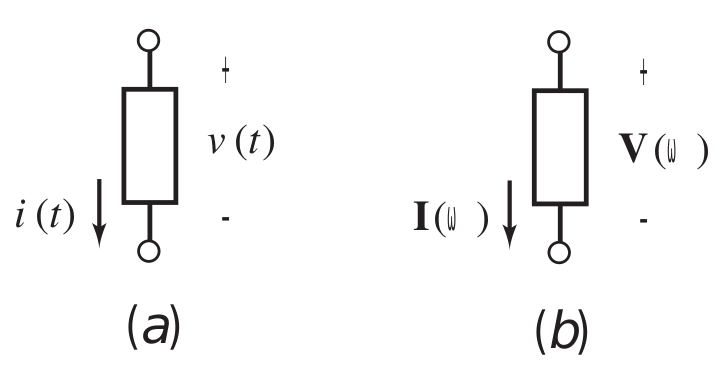
\includegraphics[width=4cm,height=2.8cm]{figure7.png}\\
An element of an
ac circuit represented (a) in the time
domain and (b) in the frequency
domain.
\end{column}
	\end{columns}\\	
\end{tabular}
\end{frame}
% ----------------- NOVO SLIDE --------------------------------
\begin{frame}[fragile]
	\frametitle{Impedances}
\begin{tabular}{ll}

	\begin{columns}
	\begin{column}{.33\textwidth}  %%<--- here
\center 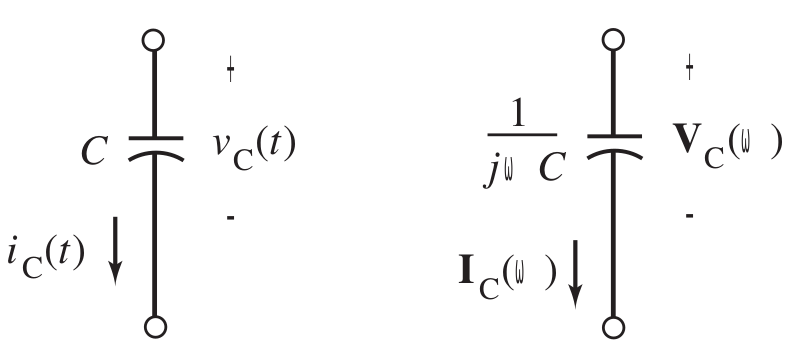
\includegraphics[width=4cm,height=2.8cm]{figure8.png}\\			
	\end{column}
	\begin{column}{.33\textwidth}  %%<--- here
\center 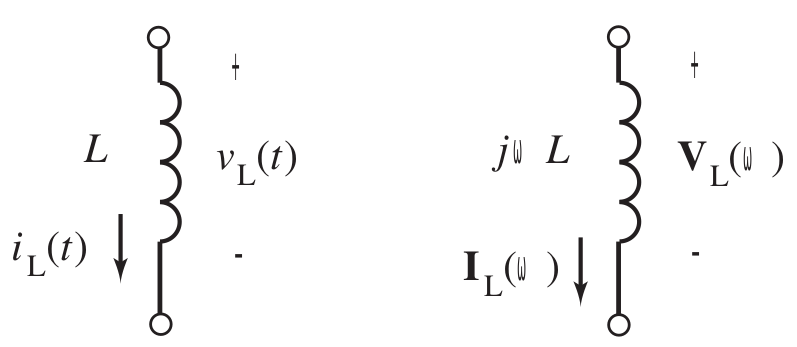
\includegraphics[width=4cm,height=2.8cm]{figure9.png}\\			
	\end{column}
	\begin{column}{.33\textwidth}  %%<--- here
\center 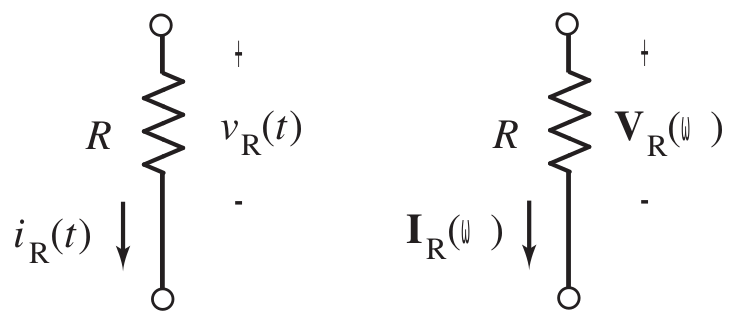
\includegraphics[width=4cm,height=2.8cm]{figure10.png}\\			
	\end{column}
	\end{columns}\\
	\begin{columns}
\scriptsize	\begin{column}{.33\textwidth}  %%<--- here
\newline \\ $ v_C(t)=A \cos(\omega t + \theta)$ \\ $\Rightarrow  \textbf{V}_C(\omega) = A \angle{\theta}$\\	
$ i_C(t)= C\frac{d}{dt}v_C(t) = A \omega C \cos(\omega t + \theta +90^o)$ \\ $\Rightarrow  \textbf{I}_C(\omega) = jA \omega C \angle{\theta}$\\	
$$\textbf{Z}(\omega)=\dfrac{\textbf{V}(\omega)}{\textbf{I}(\omega)}=\dfrac{1}{j \omega C} \ \Omega$$
	
	\end{column}
	\begin{column}{.33\textwidth}  %%<--- here
\newline \\$ i_L(t)=A \cos(\omega t + \theta)$ \\ $\Rightarrow  \textbf{I}_L(\omega) = A \angle{\theta}$\\	
$ v_L(t)= L\frac{d}{dt}i_L(t) = A \omega L \cos(\omega t + \theta +90^o)$ \\ $\Rightarrow  \textbf{V}_L(\omega) = jA \omega L \angle{\theta}$\\	
$$\textbf{Z}(\omega)=\dfrac{\textbf{V}(\omega)}{\textbf{I}(\omega)}=j \omega L \ \Omega$$			
	\end{column}
	\begin{column}{.33\textwidth}  %%<--- here
\newline \\ $ i_R(t)=A \cos(\omega t + \theta)$ \\ $\Rightarrow  \textbf{I}_R(\omega) = A \angle{\theta}$\\	
$ v_R(t)= R \ i_R(t) = R \ A \cos(\omega t + \theta)$ \\ $\Rightarrow  \textbf{V}_R(\omega) = A  R \ \angle{\theta}$\\	
$$\textbf{Z}(\omega)=\dfrac{\textbf{V}(\omega)}{\textbf{I}(\omega)}=R \ \Omega$$			
	\end{column}
	\end{columns}\\

\end{tabular}	
\end{frame}
% ----------------- NOVO SLIDE --------------------------------
\begin{frame}[fragile]
	\frametitle{Impedances}
\begin{tabular}{ll}
	\begin{columns}
		\begin{column}{1\textwidth}  %%<--- here
		\textbf{EXAMPLE 10.4-1} - The input to the ac circuit shown in Figure below is the source voltage $v_s(t)=12 \cos(1000t+15^o) \ V$.
		Detemine (a) the impedances of the capacitor, inductor, and resistance and (b) the corrent i(t).

		\begin{center}
    			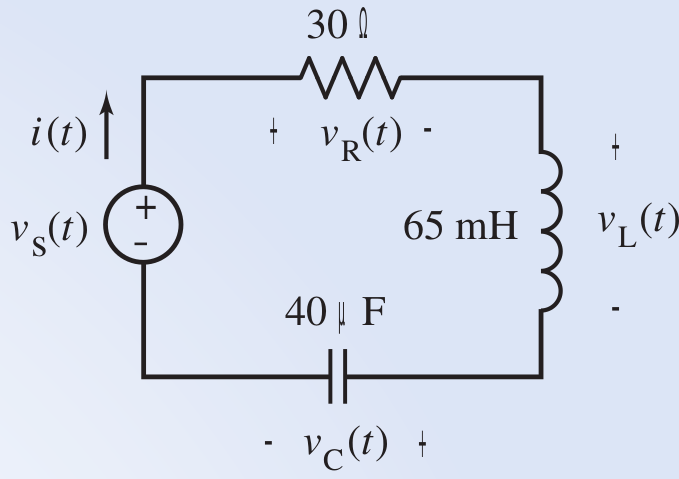
\includegraphics[height=3cm]{figure11.png}	
		\end{center}	
		\scalebox{0.8}{Answer: $\textbf{Z}_c(\omega)=-j25\ \Omega$, $\textbf{Z}_L(\omega)= j65\ \Omega$, $\textbf{Z}_R(\omega)= 30\ \Omega$, and $i(t)=0.24 \cos(1000t-38.13^o)\ A$}
		\end{column}
	\end{columns}
\end{tabular}	
\end{frame}
% ----------------- NOVO SLIDE --------------------------------
\begin{frame}[fragile]
	\frametitle{Impedances}
\begin{tabular}{ll}
	\begin{columns}
		\begin{column}{1\textwidth}  %%<--- here
		\textbf{EXAMPLE 10.4-2} - The input to the ac circuit shown in Figure below is the source voltage $v_s(t)=48 \cos(500t+75^o) \ V$.
		Detemine  the voltage v(t).

		\begin{center}
    			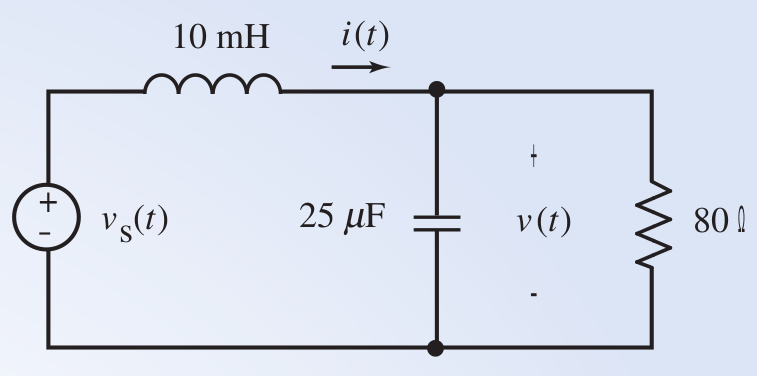
\includegraphics[height=3cm]{figure12.png}	
		\end{center}	
		\scalebox{0.8}{Answer: $v(t)=65.9 \cos(500t+16^o)\ V$}
		\end{column}
	\end{columns}
\end{tabular}	
\end{frame}
% ----------------- NOVO SLIDE --------------------------------
\begin{frame}[fragile]
	\frametitle{Impedances}
\begin{tabular}{ll}
	\begin{columns}
		\begin{column}{1\textwidth}  %%<--- here
		\textbf{EXAMPLE 10.4-2} - The input to the ac circuit shown in Figure below is the source voltage $v_s(t)=12 \cos(1000t+45^o) \ V$.
		Detemine  the voltage $v_o(t)$.

		\begin{center}
    			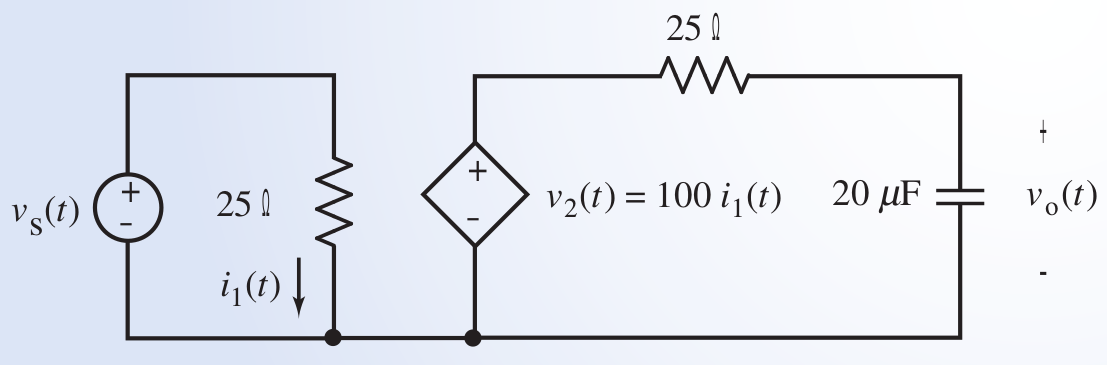
\includegraphics[height=3cm]{figure13.png}	
		\end{center}	
		\scalebox{0.8}{Answer: $v_o(t)=42.933 \cos(1000t+18.44^o)\ V$}
		\end{column}
	\end{columns}
\end{tabular}	
\end{frame}
% ----------------- NOVA SECÇÂO -----------------------------
\section{Series and Parallel Impedances (10.5)}
% ----------------- NOVO SLIDE --------------------------------

\begin{frame}[fragile]
	\frametitle{Series, Parallel Impedances and Voltage, Current Division  }
\begin{tabular}{ll}
	\begin{columns}
		\begin{column}{1\textwidth}  %%<--- here

\begin{tabular}{ll}

	\begin{columns}
	\begin{column}{.25\textwidth}  %%<--- here
 \center Series Impedances \newline \\
 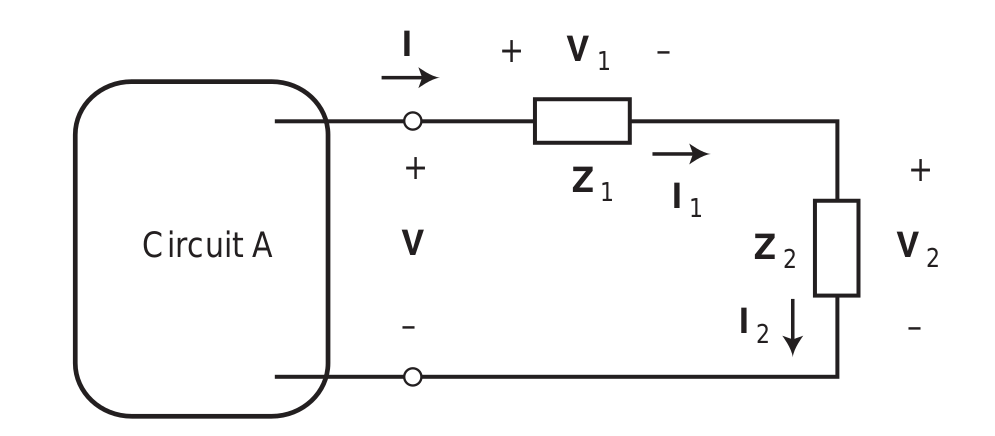
\includegraphics[width=3cm,height=2.4cm]{figure14.png}\\			
	\end{column}
	\begin{column}{.25\textwidth}  %%<--- here
\center Parallel Impedances \newline \\
 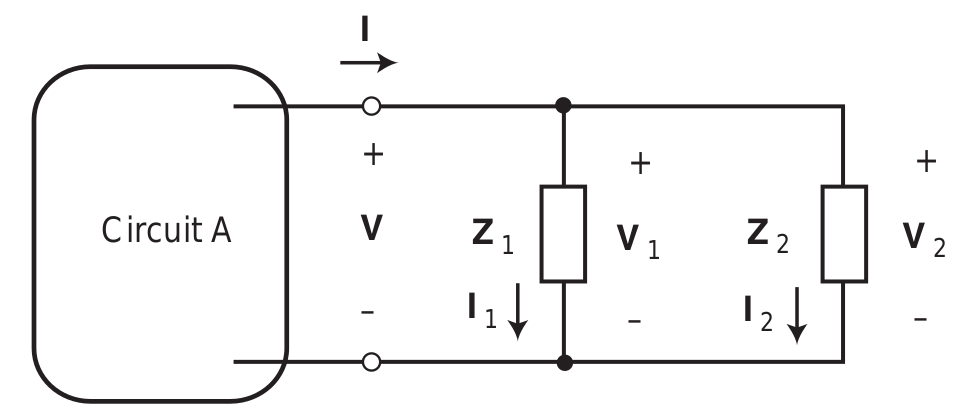
\includegraphics[width=3cm,height=2.4cm]{figure15.png}\\			
	\end{column}
	\begin{column}{.25\textwidth}  %%<--- here
\center Voltage Division \newline \\
 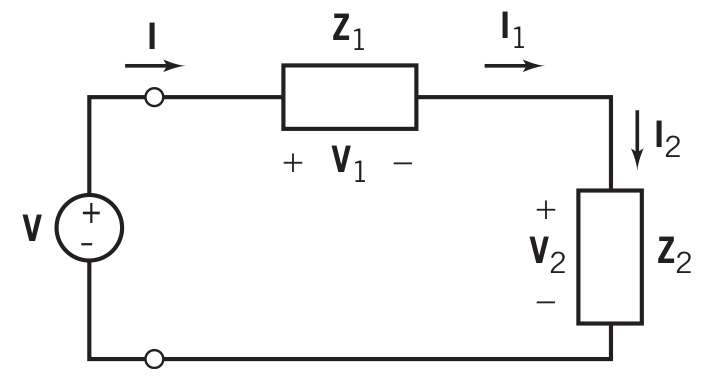
\includegraphics[width=3cm,height=2.4cm]{figure16.png}\\			
	\end{column}
	\begin{column}{.25\textwidth}  %%<--- here
\center Current Division \newline \\
 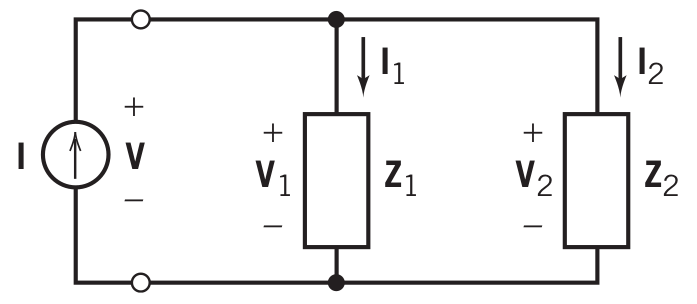
\includegraphics[width=3cm,height=2.4cm]{figure17.png}\\			
	\end{column}
	\end{columns}\\
	\begin{columns}
	\begin{column}{.25\textwidth}  %%<--- here
$$\textbf{Z}_{eq}=\textbf{Z}_1+\textbf{Z}_2$$			
	\end{column}
	\begin{column}{.25\textwidth}  %%<--- here
$$\textbf{Z}_{eq}=\dfrac{\textbf{Z}_1\textbf{Z}_2}{\textbf{Z}_1+\textbf{Z}_2}$$			
	\end{column}
	\begin{column}{.25\textwidth}  %%<--- here
$$\textbf{V}_2=\dfrac{\textbf{Z}_2}{\textbf{Z}_1+\textbf{Z}_2}V$$		
	\end{column}
	\begin{column}{.25\textwidth}  %%<--- here
$$\textbf{I}_2=\dfrac{\textbf{Z}_1}{\textbf{Z}_1+\textbf{Z}_2}I$$			
	\end{column}
	\end{columns}\\

\end{tabular}	
\end{column}

	\end{columns}
	
\end{tabular}	
\end{frame}

% ----------------- NOVO SLIDE --------------------------------
\begin{frame}[fragile]
	\frametitle{Impedances}
\begin{tabular}{ll}
	\begin{columns}
		\begin{column}{1\textwidth}  %%<--- here
		\textbf{EXAMPLE 10.5-1} - Determine the steady-state current $i(t)$ in the RLC circuit shown in Figure below, using phasors and impedances.

		\begin{center}
    			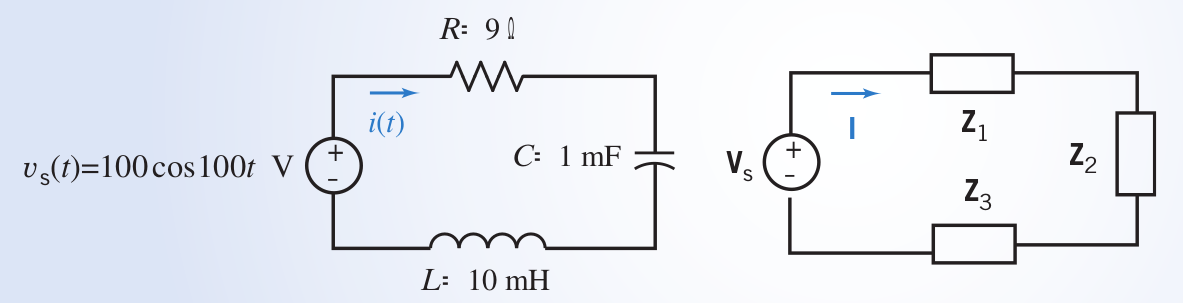
\includegraphics[height=3cm]{figure18.png}	
		\end{center}	
		\scalebox{0.8}{Answer: $i(t)=7.86 \cos(100t+45^o)\ A$}
		\end{column}
	\end{columns}
\end{tabular}	
\end{frame}
% ----------------- NOVO SLIDE --------------------------------
\begin{frame}[fragile]
	\frametitle{Impedances}
\begin{tabular}{ll}
	\begin{columns}
		\begin{column}{.5\textwidth}  %%<--- here
		\textbf{EXAMPLE 10.5-4} - Consider the circuit shown in Figure below. The input
to the circuit is the voltage of the voltage source $v_s(t)$,
and the output is the voltage across the $4 \ \Omega$ resistor,
$v_o(t)$. When the input is $v_s(t)=8.93 \cos(2t+54^o)\ V$,
the corresponding output is $v_o(t)=3.83 \cos(2t+83^o)\ V$. Determine the voltage across the $9\ \Omega$
resistor $v_a(t)$ and the value of the capacitance $C$ of the
capacitor.
	

		\end{column}
				\begin{column}{.5\textwidth}  %%<--- here

		\begin{center}
    			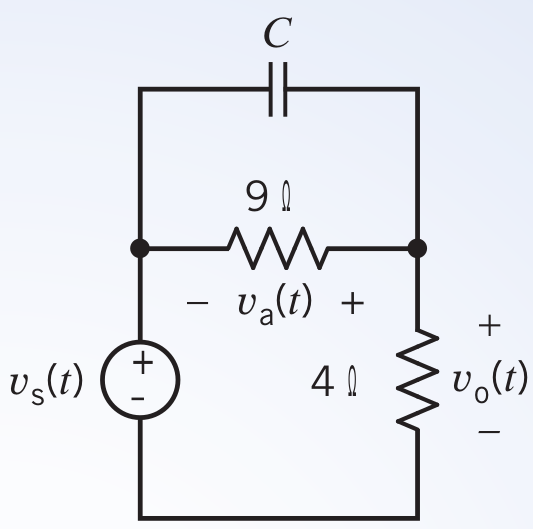
\includegraphics[height=4.5cm]{figure19.png}	
		\end{center}	
		\scalebox{0.8}{Answer: $v_a(t)=5.88 \cos(2t+216^o)\ V$ and $C=60mF.$}
		\end{column}
	\end{columns}
\end{tabular}	
\end{frame}
% ----------------- NOVA SECÇÂO -----------------------------
\section{Mesh and Node Equations (10.6)}
% ----------------- NOVO SLIDE --------------------------------
\begin{frame}[fragile]
	\frametitle{Node Equations }
\begin{tabular}{ll}
	\begin{columns}
\small		\begin{column}{.7\textwidth}  %%<--- here
		The node equations are a set of simultaneous equations in which the unknowns are the node
voltages. We write the node equations by
	\begin{enumerate}
	\item {Expressing the element voltages and currents (for example, the current and voltage of an
impedance) in terms of the node voltages.}
	\item {Applying KCL at the nodes of the ac circuit.}		
	\end{enumerate}
After writing and solving the node equations, we can determine all of the voltages and currents of the ac
circuit using Ohm’s and Kirchhoff’s laws.
		\end{column}
		\begin{column}{.3\textwidth}  %%<--- here
		\begin{center}
    			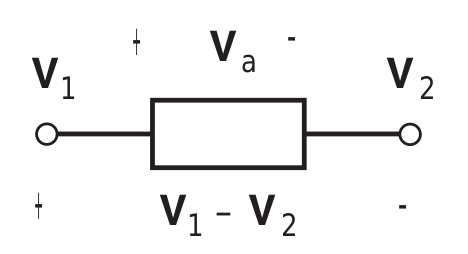
\includegraphics[height=1.5cm]{figure20.png}\\
    			    			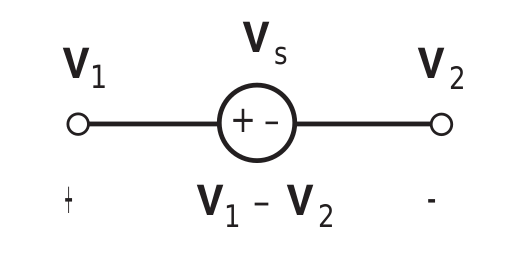
\includegraphics[height=1.5cm]{figure21.png}\\
    			    			    			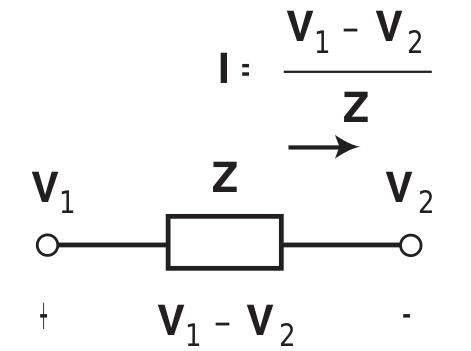
\includegraphics[height=2cm]{figure22.png}
		\end{center}	
		
		\end{column}
	\end{columns}
\end{tabular}	
\end{frame}
% ----------------- NOVO SLIDE --------------------------------
\begin{frame}[fragile]
	\frametitle{Node Equations }
\begin{tabular}{ll}
	\begin{columns}
		\begin{column}{1\textwidth}  %%<--- here
		\textbf{EXAMPLE 10.6-1} - Determine the voltage $v_a(t)$ for the circuit shown in Figure below.

		\begin{center}
    			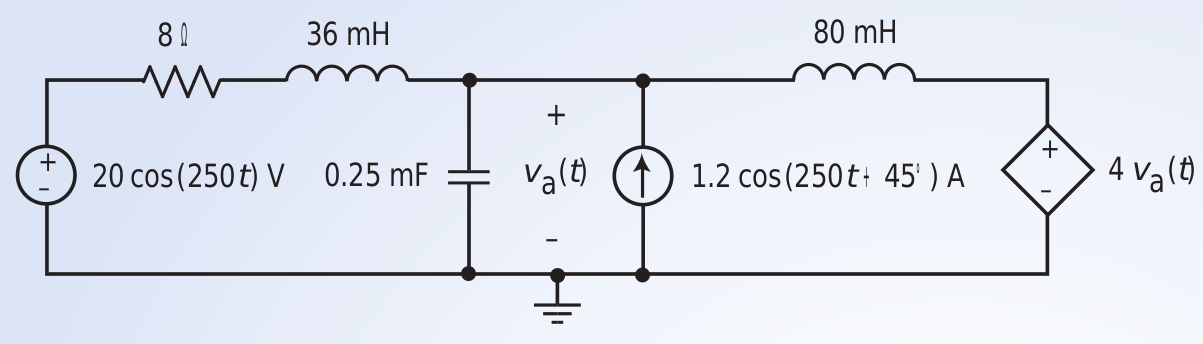
\includegraphics[height=3cm]{figure23.png}	
		\end{center}	
		\scalebox{0.8}{Answer: $v_a(t)=12.43 \cos(250t+81.2^o)\ V$}
		\end{column}
	\end{columns}
\end{tabular}	
\end{frame}
% ----------------- NOVO SLIDE --------------------------------
\begin{frame}[fragile]
	\frametitle{Mesh Equation}
\begin{tabular}{ll}
	\begin{columns}
\small		\begin{column}{.7\textwidth}  %%<--- here
		The mesh equations are a set of simultaneous equations in which the unknowns are the mesh
currents. We write the mesh equations by
	\begin{enumerate}
	\item {Expressing the element voltages and currents (for example, the current and voltage of an
impedance) in terms of the mesh currents.}
	\item {Applying KVL to the meshes of the ac circuit.}		
	\end{enumerate}
After writing and solving the mesh equations, we can determine all of the voltages and currents of the ac
circuit using Ohm’s and Kirchhoff’s laws.
		\end{column}
		\begin{column}{.3\textwidth}  %%<--- here
		\begin{center}
    			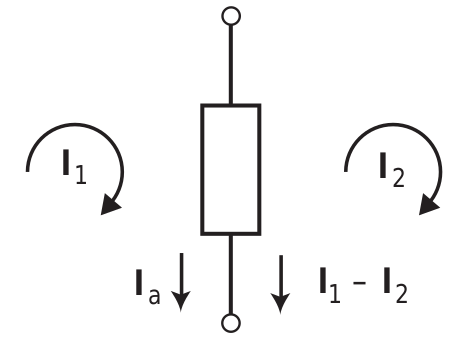
\includegraphics[height=2cm]{figure24.png}\\
    			    			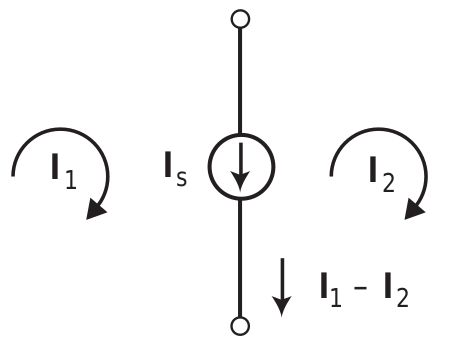
\includegraphics[height=2cm]{figure25.png}\\
    			    			    			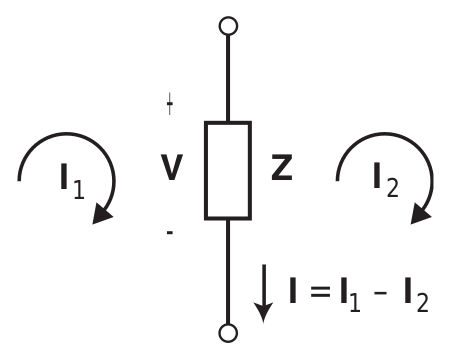
\includegraphics[height=2cm]{figure26.png}
		\end{center}	
		
		\end{column}
	\end{columns}
\end{tabular}	
\end{frame}
% ----------------- NOVO SLIDE --------------------------------
\begin{frame}[fragile]
	\frametitle{Mesh Equations }
\begin{tabular}{ll}
	\begin{columns}
		\begin{column}{1\textwidth}  %%<--- here
		\textbf{EXAMPLE 10.6-2} - Determine the mesh currents for the circuit shown in Figure below.

		\begin{center}
    			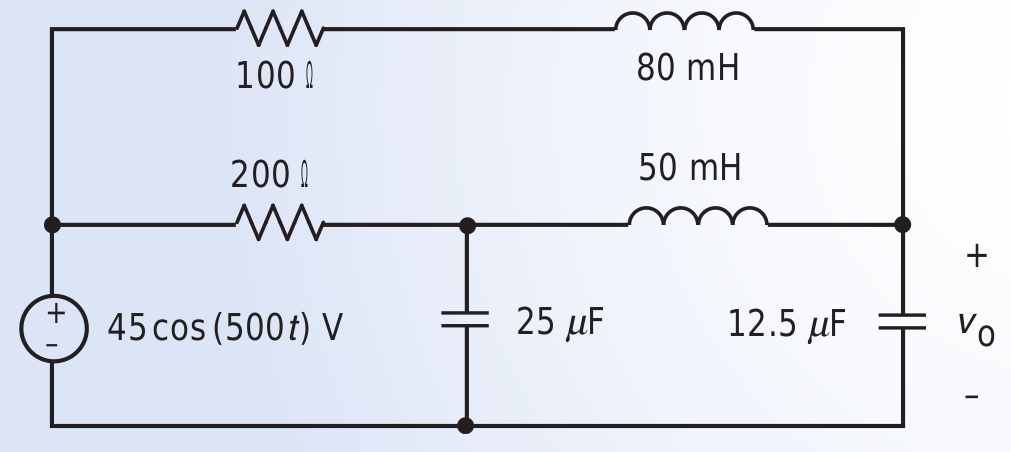
\includegraphics[height=3cm]{figure27.png}	
		\end{center}	
		\scalebox{0.6}{Answer: $i_1(t)=374 \cos(500t+15^o)\ V$,  $i_2(t)=575 \cos(500t+25^o)\ V$ and  $i_3(t)=171 \cos(500t+28^o)\ V$}
		\end{column}
	\end{columns}
\end{tabular}	
\end{frame}
% ----------------- NOVO SLIDE --------------------------------
\begin{frame}[fragile]
	\frametitle{Mesh Equations }
\begin{tabular}{ll}
	\begin{columns}
		\begin{column}{1\textwidth}  %%<--- here
		\textbf{EXAMPLE 10.6-4} - The input to the ac circuit shown in Figure below is the
voltage source voltage $v_s(t)=125 \cos(500 t + 15^o) \ mV$. Determine the output voltage $v_o (t)$.

		\begin{center}
    			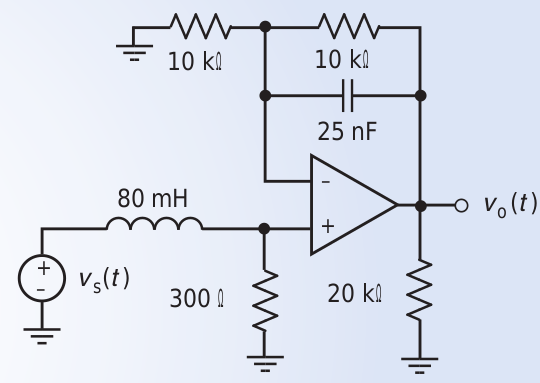
\includegraphics[height=3cm]{figure28.png}	
		\end{center}	
		\scalebox{0.6}{Answer: $v_o(t)=174 \cos(500t+69.79^o)\ mV$}
		\end{column}
	\end{columns}
\end{tabular}	
\end{frame}
% ----------------- NOVA SECÇÂO -----------------------------
\section{Thevenin and Norton Equivalent Circuits (10.7)}
% ----------------- NOVO SLIDE --------------------------------
\begin{frame}[fragile]
%	\frametitle{Initial Value Theorems }
\begin{tabular}{ll}
	\begin{columns}
		\begin{column}{1\textwidth}  %%<--- here

\begin{tabular}{ll}
	\begin{columns}
	\begin{column}{1\textwidth}  %%<--- here

 \footnotesize The open-circuit voltage $\textbf{V}_{oc}$ , the short-circuit current $\textbf{I}_{sc}$, and the Thevenin impedance $\textbf{Z}_{t}$, are
related by the equation $\textbf{V}_{oc}=\textbf{Z}_{t} \ \textbf{I}_{sc}$.		
	\end{column}


	\end{columns}\\
	\begin{columns}
	\begin{column}{.33\textwidth}  %%<--- here

 \center 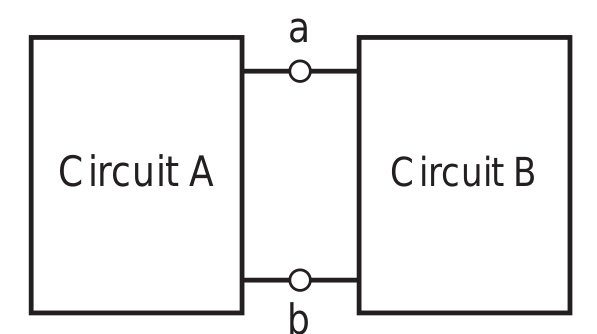
\includegraphics[width=3cm,height=2cm]{figure29.png}\\ \tiny Circuit A and Circuit B.			
	\end{column}
	\begin{column}{.33\textwidth}  %%<--- here

  \center 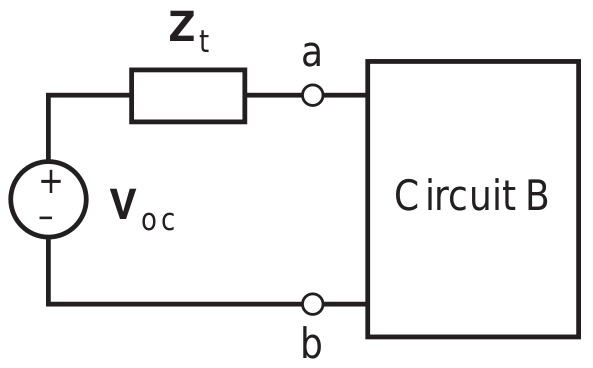
\includegraphics[width=3cm,height=2cm]{figure30.png}\\ \tiny Thevenin equivalent circuit.			
	\end{column}
	\begin{column}{.33\textwidth}  %%<--- here

  \center 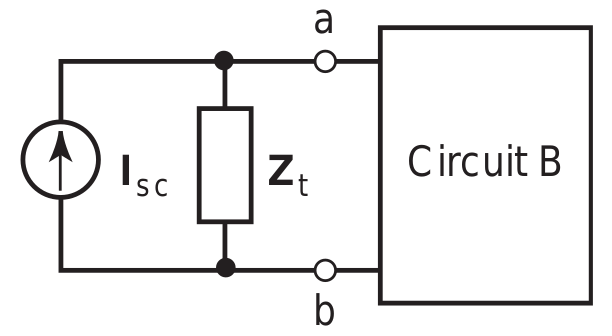
\includegraphics[width=3cm,height=2cm]{figure31.png}\\  \tiny Norton equivalent circuit.			
	\end{column}

	\end{columns}\\
		\begin{columns}
	\begin{column}{1\textwidth}  %%<--- here

 \footnotesize The Thevenin equivalent
circuit involves three parameters:			
	\end{column}


	\end{columns}\\
	
	
	\begin{columns}
	\begin{column}{.33\textwidth}  %%<--- here

\center  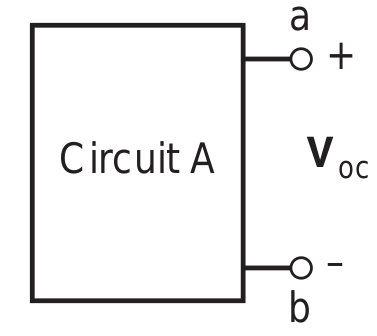
\includegraphics[width=3cm,height=2cm]{figure32.png}\\ \tiny The open-circuit voltage $\textbf{V}_{oc}$			
	\end{column}
	\begin{column}{.33\textwidth}  %%<--- here

  \center 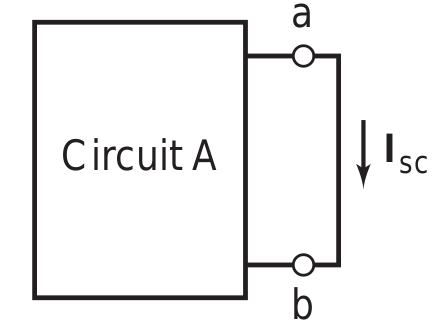
\includegraphics[width=3cm,height=2cm]{figure33.png}\\ \tiny The short-circuit current $\textbf{I}_{sc}$			
	\end{column}
	\begin{column}{.33\textwidth}  %%<--- here

  \center 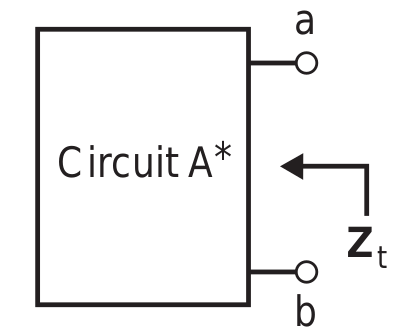
\includegraphics[width=3cm,height=2cm]{figure34.png}\\ \tiny The Thevenin impedance $\textbf{Z}_{t}$			
	\end{column}

	\end{columns}\\

\end{tabular}	
\end{column}

	\end{columns}
	
\end{tabular}		
\end{frame}

% ----------------- NOVO SLIDE --------------------------------
\begin{frame}[fragile]
	\frametitle{Thevenin Equivalent Circuit }
\begin{tabular}{ll}
	\begin{columns}
		\begin{column}{1\textwidth}  %%<--- here
		\textbf{EXAMPLE 10.7-1} - Find the Thevenin equivalent circuit of the ac circuit in Figure shown below.

		\begin{center}
    			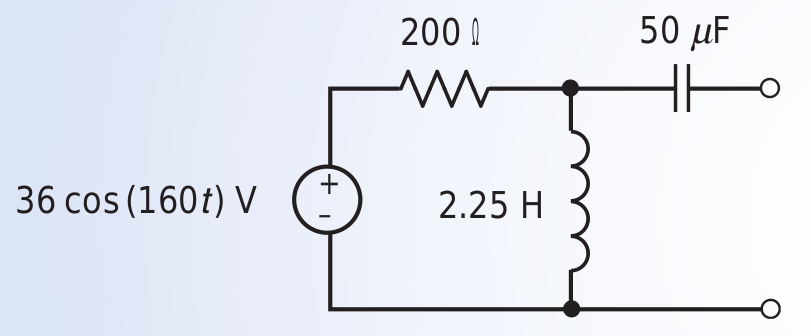
\includegraphics[height=3cm]{figure35.png}	
		\end{center}	
		\scalebox{0.6}{Answer: $\textbf{V}_{oc}=31.47 \angle{29.1^o}\ V$  \ and \ $\textbf{Z}_{t}=152.83-j40.094 \ \Omega$}
		\end{column}
	\end{columns}
\end{tabular}	
\end{frame}
% ----------------- NOVO SLIDE --------------------------------
\begin{frame}[fragile]
	\frametitle{Norton Equivalent Circuit }
\begin{tabular}{ll}
	\begin{columns}
		\begin{column}{1\textwidth}  %%<--- here
		\textbf{EXAMPLE 10.7-2} - Find the Norton equivalent circuit of the ac circuit in Figure shown below.

		\begin{center}
    			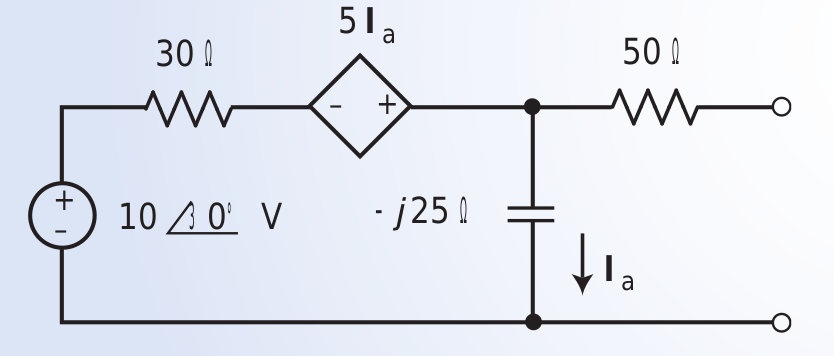
\includegraphics[height=3cm]{figure36.png}	
		\end{center}	
		\scalebox{0.6}{Answer: $\textbf{I}_{sc}=0.11 \angle{-2.01^o}\ A$  \ and \ $\textbf{Z}_{n}=66 \angle{-13^0} \ \Omega$}
		\end{column}
	\end{columns}
\end{tabular}	
\end{frame}



% ----------------- NOVA SECÇÂO -----------------------------
\section{Superposition (10.8)}
% ----------------- NOVO SLIDE --------------------------------
\begin{frame}[fragile]
	\frametitle{Superposition}
\begin{tabular}{ll}
	\begin{columns}
		\begin{column}{1\textwidth}  %%<--- here
		\textbf{EXAMPLE 10.8-1} - Determine the voltage $v_o(t)$ across the $8 \Omega$ resistor in the circuit shown below.

		\begin{center}
    			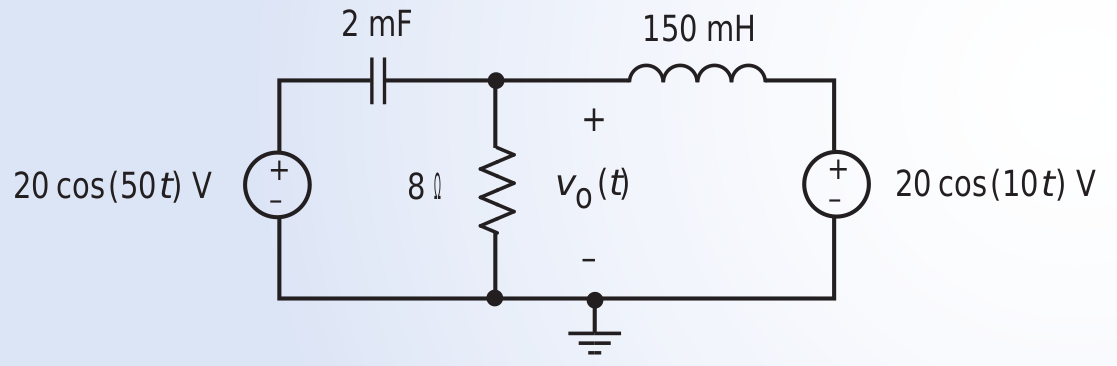
\includegraphics[height=3cm]{figure37.png}	
		\end{center}	
		\scalebox{0.6}{Answer: $v_o(t)=v_{o1}(t)+v_{o2}(t)=15.46 \cos(50t+104.0^o)+20.24 \cos(10t-10.94^o)$}
		\end{column}
	\end{columns}
\end{tabular}	
\end{frame}
% ----------------- NOVA SECÇÂO -----------------------------
\section{Phasor Diagrams (10.9)}
% ----------------- NOVO SLIDE --------------------------------
\begin{frame}[fragile]
%	\frametitle{Initial Value Theorems }
\begin{tabular}{ll}
	\begin{columns}
	\begin{column}{1\textwidth}  %%<--- here

 \footnotesize A \textbf{phasor diagram} is a graphical representation of phasors and their relationship on the
complex plane.	
	\end{column}


	\end{columns}\\
	\begin{columns}
	\begin{column}{.33\textwidth}  %%<--- here

 \center 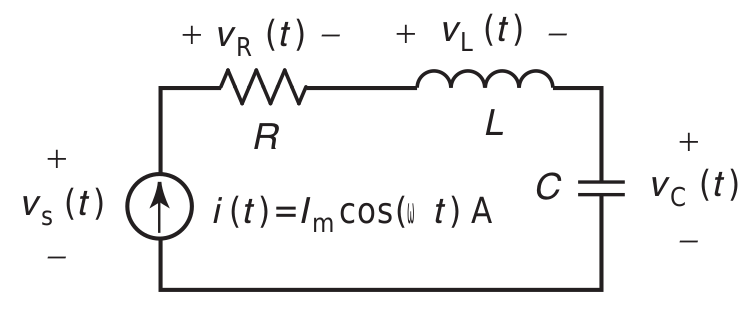
\includegraphics[width=3cm,height=2cm]{figure38.png}\\ \tiny The time domain			
	\end{column}
	\begin{column}{.33\textwidth}  %%<--- here

  \center 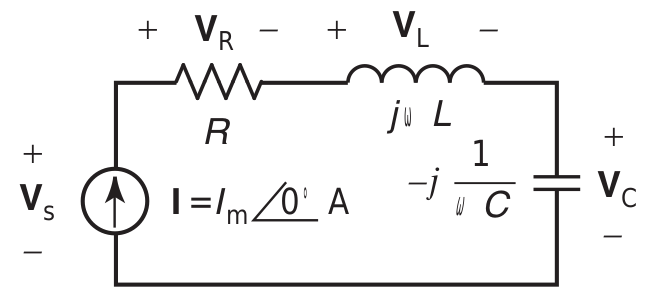
\includegraphics[width=3cm,height=2cm]{figure39.png}\\ \tiny The frequency domain			
	\end{column}
	\begin{column}{.33\textwidth}  %%<--- here
\footnotesize Equations:\\
$\textbf{I}_{m}={I}_{m}\angle{0^o}$\\
$\textbf{V}_{R}=RI_{m}\angle{0^o}$\\
$\textbf{V}_{L}=j\omega L (I_{m}\angle{0})=\omega L I_{m}\angle{90^o}$\\
$\textbf{V}_{C}=\frac{1}{j\omega C} (I_{m}\angle{0})=\frac{I_{m}}{\omega C} \angle{-90^o}$\\
$\textbf{V}_{S}=\textbf{V}_{R}+\textbf{V}_{L}+\textbf{V}_{C}$\\

	
	
  			
	\end{column}

	\end{columns}\\
		\begin{columns}
	\begin{column}{1\textwidth}  %%<--- here

 \footnotesize Phasor diagrams for the RLC circuit in Figure above			
	\end{column}


	\end{columns}\\
	
	
	\begin{columns}
	\begin{column}{.33\textwidth}  %%<--- here

\center  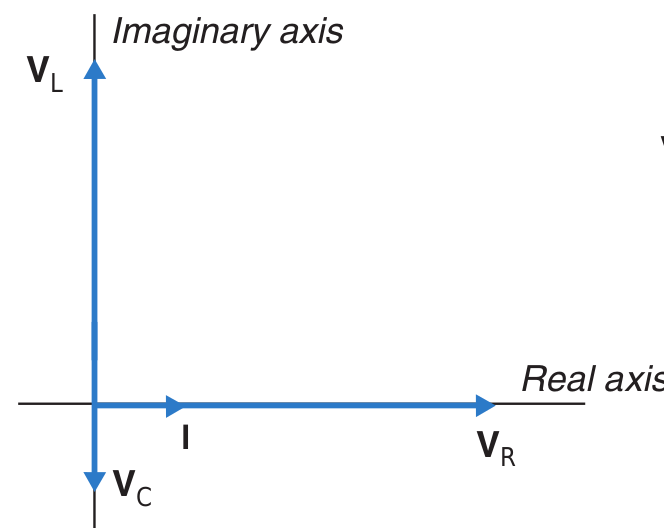
\includegraphics[width=3cm,height=2cm]{figure40.png}\\ 			
	\end{column}
	\begin{column}{.33\textwidth}  %%<--- here

  \center 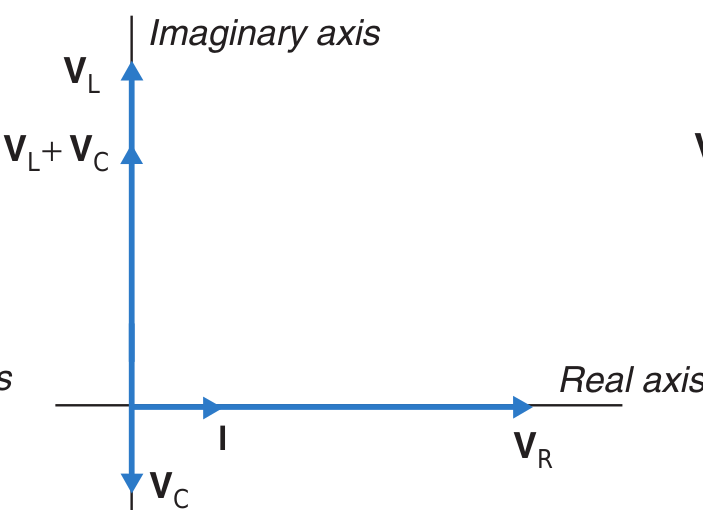
\includegraphics[width=3cm,height=2cm]{figure41.png}\\ 			
	\end{column}
	\begin{column}{.33\textwidth}  %%<--- here

  \center 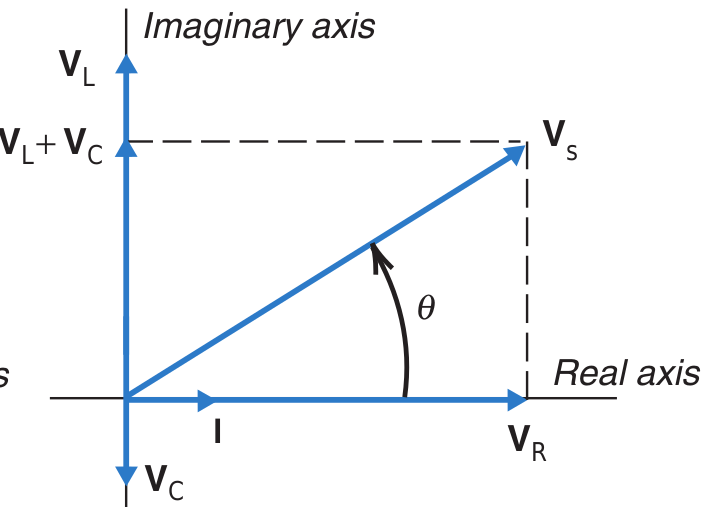
\includegraphics[width=3cm,height=2cm]{figure42.png}\\ 			
	\end{column}

	\end{columns}\\

\end{tabular}		
\end{frame}
% ----------------- NOVO SLIDE --------------------------------
\begin{frame}[fragile]
	\frametitle{Phasor Diagrams}
\begin{tabular}{ll}
	\begin{columns}
		\begin{column}{1\textwidth}  %%<--- here
		\textbf{EXAMPLE 10.9-1} - Consider the circuit shown in Figure below when $R = 80 \Omega$, $L = 8 H$, $C = 5 mF$ and
$i(t)=0.25 \cos(10t) \ A$. Determine the phasor diagram.

		\begin{center}
    			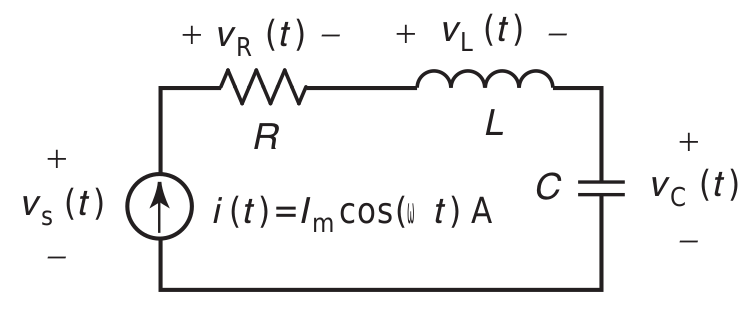
\includegraphics[height=3cm]{figure38.png}	
		\end{center}	
		\scalebox{0.6}{Answer: $\textbf{V}_{R}=20 \angle{0^o}\ V$, $\textbf{V}_{L}=20 \angle{90^o}\ V$, $\textbf{V}_{C}=5 \angle{-90^o}\ V$ and $\textbf{V}_{S}=25 \angle{36.9^o}\ V$ }
		\end{column}
	\end{columns}
\end{tabular}	
\end{frame}

% ----------------- NOVA SECÇÂO -----------------------------
\section{Op Amps in AC Circuits (10.10)}
% ----------------- NOVO SLIDE --------------------------------
\begin{frame}[fragile]
	\frametitle{Op Amps}
\begin{tabular}{ll}
	\begin{columns}
		\begin{column}{1\textwidth}  %%<--- here
		\textbf{EXAMPLE 10.10-1} - Find the ratio ${\textbf{V}_{o}}/{\textbf{V}_{i}}$ for the circuit of Figure below when $R_1 = 1\ kV$, $R_2 = 10 \ kV$, $C_1 = 0\ F$, and 
		$C_2 = 0.1\ \mu F$ for $\omega = 1000\ rad/s$.

		\begin{center}
    			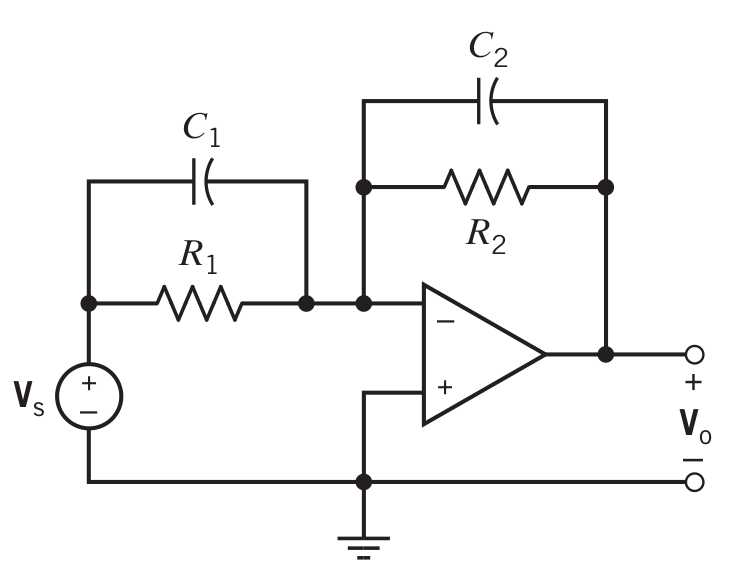
\includegraphics[height=3.5cm]{figure44.png}	
		\end{center}	
		\scalebox{0.6}{Answer: ${\textbf{V}_{o}}/{\textbf{V}_{i}}=7.07 \angle{135^o}$}
		\end{column}
	\end{columns}
\end{tabular}	
\end{frame}
% ----------------- NOVA SECÇÂO -----------------------------
\section{The Complete Response (10.11)}
% ----------------- NOVO SLIDE --------------------------------
\begin{frame}[fragile]
	\frametitle{The Complete Response}
\begin{tabular}{ll}
	\begin{columns}
		\begin{column}{1\textwidth}  %%<--- here
		Next, we consider circuits with sinusoidal inputs that are subject to abrupt changes, as when a switch
opens or closes. To find the complete response of such circuits, we: \newline \\
		\begin{itemize}
\item[$\clubsuit$]{Represent the circuit by a differential equation.}
\item[$\clubsuit$]{Find the general solution of the homogeneous differential equation.}
\item[$\clubsuit$]{Find a particular solution of the differential equation.}
\item[$\clubsuit$]{Represent the response of the circuit as $v(t)=v_n(t)+v_f(t)$.}	
\item[$\clubsuit$]{Use the initial conditions to evaluate the unknown constants.}
	
					\end{itemize}
\end{column}

	\end{columns}
	
\end{tabular}	
\end{frame}

% ----------------- NOVO SLIDE --------------------------------
\begin{frame}[fragile]
	\frametitle{The Complete Response}
\begin{tabular}{ll}
	\begin{columns}
		\begin{column}{1\textwidth}  %%<--- here
		\textbf{EXAMPLE 10.11-1} - Determine $v(t)$, the voltage across the capacitor in Figure below, both before and after the switch closes.

		\begin{center}
    			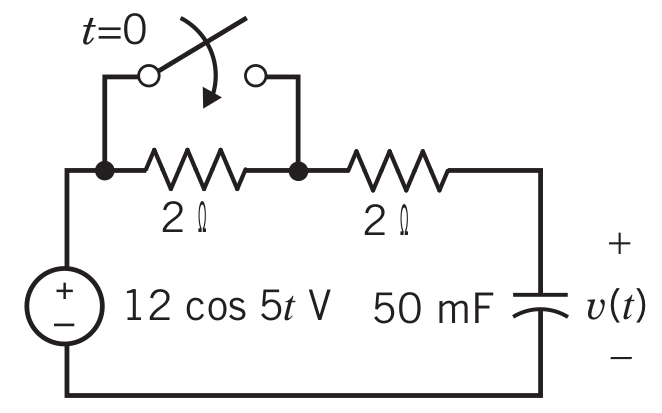
\includegraphics[height=3cm]{figure43.png}	
		\end{center}	
		\scalebox{0.6}{Answer: $
	    v(t)=
	    \begin{cases}
	    8.49 \cos(5t-45^o), \ when \ t < 0 \\
	%    \newline \\
	     -3.6e^{-10t}+10.74 \cos(5t-26.6^o), \ when \ t > 0 \\
	    
	    \end{cases}
	    $ }
		\end{column}
	\end{columns}
\end{tabular}	
\end{frame}


\end{document} 

